\documentclass{article}


% if you need to pass options to natbib, use, e.g.:
%     \PassOptionsToPackage{numbers, compress}{natbib}
% before loading neurips_2023


% ready for submission
\usepackage[nonatbib]{neurips_2023}



% to compile a preprint version, e.g., for submission to arXiv, add add the
% [preprint] option:
%     \usepackage[preprint]{neurips_2023}


% to compile a camera-ready version, add the [final] option, e.g.:
%     \usepackage[final]{neurips_2023}


% to avoid loading the natbib package, add option nonatbib:
%    \usepackage[nonatbib]{neurips_2023}


\usepackage[utf8]{inputenc} % allow utf-8 input
\usepackage[T1]{fontenc}    % use 8-bit T1 fonts
\usepackage{hyperref}       % hyperlinks
\usepackage{url}            % simple URL typesetting
\usepackage{booktabs}       % professional-quality tables
\usepackage{amsfonts}       % blackboard math symbols
\usepackage{nicefrac}       % compact symbols for 1/2, etc.
\usepackage{microtype}      % microtypography
\usepackage{xcolor}         % colors
\usepackage{adjustbox}

\usepackage{graphicx} % For \includegraphics
\usepackage{subcaption} % For subfigures and subcaptions
% \usepackage{float} % Optional, for more control over figure placement e.g. [H]
\title{Automated Kelp Canopy Mapping: A UNet Approach with Landsat \& Citizen Science}


% The \author macro works with any number of authors. There are two commands
% used to separate the names and addresses of multiple authors: \And and \AND.
%
% Using \And between authors leaves it to LaTeX to determine where to break the
% lines. Using \AND forces a line break at that point. So, if LaTeX puts 3 of 4
% authors names on the first line, and the last on the second line, try using
% \AND instead of \And before the third author name.


\author{%
  Maxwell Rehm\thanks{Special Thanks to my Advisors Alexander C. Berg and Nadia Ahmed} \\
  ICS Honors | Campuswide Honors Collegium \\
  University of California, Irvine\\
  % examples of more authors
  % \And
  % Coauthor \\
  % Affiliation \\
  % Address \\
  % \texttt{email} \\
  % \AND
  % Coauthor \\
  % Affiliation \\
  % Address \\
  % \texttt{email} \\
  % \And
  % Coauthor \\
  % Affiliation \\
  % Address \\
  % \texttt{email} \\
  % \And
  % Coauthor \\
  % Affiliation \\
  % Address \\
  % \texttt{email} \\
}


\begin{document}


\maketitle


\begin{abstract}
  Automated, cost-effective monitoring of kelp forests is crucial for understanding and mitigating the ongoing kelp crisis driven by urchin overpopulation, as it enables targeted diver interventions. Previous studies have established methods for kelp mapping using aerial surveys, UAVs, and satellite-based spectral unmixing (MESMA), alongside the development of citizen science initiatives like Floating Forests which provide noise-robust, human-consensus labels from Landsat imagery. This study developed and evaluated an end-to-end deep learning pipeline, utilizing a UNet architecture with pre-trained ResNet backbones, for semantic segmentation of kelp canopy in Landsat 7 imagery using these Floating Forests labels, incorporating rigorous data preprocessing and augmentation. We found that a ResNet34 backbone, trained on cleaned and augmented data, achieved an Intersection over Union (IoU) of 0.5028, with data preprocessing and augmentation proving essential for optimal performance. Our study suggests that deep learning, leveraged with citizen-science-derived ground truth, offers a viable and scalable approach to automate kelp canopy mapping, which can enhance the efficiency of conservation efforts by reallocating resources towards direct ecological interventions.
\end{abstract}


\section{Introduction}

\subsection{The Kelp Crisis}

California is currently experiencing a devastating die-off of its kelp forests, a crisis largely attributed to an explosion in pacific purple sea urchin populations. This urchin surge began after their natural predator, the sunflower sea star, suffered a decline due to sea star wasting syndrome, which emerged around 2013. The disease pushed the sunflower sea star to the brink of extinction, leading to its current critically endangered status. With their primary predator virtually gone, purple sea urchin populations have exploded. These unchecked urchins, which feed on kelp, are now responsible for the destruction of vast kelp forests. Estimates indicate an 80\% loss in Northern California since 2013 (Zuckerman, 2023).

\subsection{The Need for Intervention} 

Intervention through manual urchin destruction by divers is possible, but the scarcity of these skilled individuals demands an efficient allocation strategy. The West Coast Region Kelp Team underscores this by calling for an efficient way to "conduct annual assessments of kelp forest ecosystem health" (Hohman et al., 2023, p. 5). The rationale is straightforward: areas identified with poor kelp health are likely to harbor high concentrations of urchins. These assessments would enable dive teams to strategically target urchin removal efforts in these compromised zones, thereby creating conditions more favorable for kelp recovery and regrowth. 

A primary approach to determining kelp forest ecosystem health involves quantifying the amount of kelp visible on the ocean's surface. By measuring this surface kelp area and consistently tracking these measurements over successive years, managers can identify significant trends. For instance, a substantial reduction in the surface area of kelp within a region that previously had extensive kelp beds is a strong indicator of a struggling ecosystem. Such temporal comparisons are therefore crucial for pinpointing areas most in need of intervention.

\subsection{Challenges with Existing Monitoring Methods and Why New Methods Are Needed} 

Current kelp monitoring techniques, such as costly scuba diver surveys, struggle with scalability. This inherent limitation in spatial coverage per dive makes it impractical to assess vast coastlines using only diver-based methods. Aerial surveys, while covering larger areas, share the issue of high cost and introduce the burden of repetitive human annotation. For example, the California Department of Fish and Wildlife annually conducts flights to photograph the ocean surface along the California coast. Scientists then manually analyze these images to perform kelp canopy mapping, a process that involves visually identifying kelp floating on the surface and meticulously calculating its total area, often expressed in square feet. This process is expensive, time-consuming, and repetitive. The high costs associated with these traditional methods divert significant financial resources that could otherwise be allocated to direct intervention efforts, such as funding more diver teams for urchin removal. This financial constraint, coupled with the labor intensity, prompts an urgent need to explore whether this kelp mapping task can be automated using more cost-effective and readily available data sources.

\subsection{Existing Digital Data and Automation Techniques for Kelp Maps} 

Several digital data sources and automation techniques exist for creating kelp maps, each with distinct advantages and limitations. The California Department of Fish and Wildlife, for instance, produces shapefiles derived from extensive aerial surveys. This process, detailed by MBC Applied Environmental Sciences (2017), involves capturing numerous photographs, manually creating photo-mosaics, and  using Geographic Information System (GIS) software for georeferencing and area calculation, making it inherently labor-intensive and time-consuming to produce.

More recently, Unoccupied Aerial Vehicles (UAVs) have been employed to map kelp canopy at high resolution. Saccomanno et al. (2022) describe a workflow for creating kelp canopy maps from UAV imagery, valuable for local-scale restoration; however, a key limitation is the extremely small spatial scale, with surveyed sites noted as varying from only "0.16 to 1.48 km²."

A more promising avenue for large-scale, cost-effective monitoring lies in utilizing Earth-observing satellite data, such as imagery from the Landsat program. This data is plentiful, regularly collected over vast areas by agencies like NASA, and is often available at low or no cost, offering a significant advantage over dedicated aerial or UAV campaigns. However, a primary drawback of satellite imagery is its inherent susceptibility to various forms of "noise" – such as atmospheric haze, sun glint on the water surface, and subtle water color variations – which can obscure or distort the appearance of kelp. 

For broader scale analysis, satellite data can be processed using techniques like Multiple Endmember Spectral Mixture Analysis (MESMA), as explored by Bell et al. (2020). MESMA leverages spectral physics and the use of pre-defined 'endmembers', which are pure materials like kelp or water, to estimate kelp cover. The idea is that any pixel is a linear combination of water and kelp. However, water itself doesn't always look the same – it might be clear, cloudy with mud, or have bright sun reflections – there are many types of water endmembers. The correct endmember must be selected in order for the MESMA process to be accurate. The paper uses an automatic selection process to choose the correct set of endmembers per image. The challenge with this fixed automation is its potential vulnerability to the aforementioned noise in satellite imagery; an incorrect endmember selection, possibly triggered by noise or poor sampling, can lead to inaccuracies in the resulting kelp maps.

\subsection{Bridging the Data Gap: Citizen Science} 

An alternative source of kelp data comes from the Floating Forests project, which offers a distinct method for generating kelp maps, addressing the challenges of interpreting noisy satellite imagery. This citizen science initiative leverages data from Earth-observing satellite programs, specifically using Landsat 7 satellite imagery of the Falkland Islands. The project demonstrated that accurate kelp maps could be constructed from the consensus of multiple untrained participants. Studies by Rosenthal et al. (2018) have validated this consensus method, showing it produces kelp maps with significant accuracy. 
        
The core strength of this approach lies in its inherent robustness to noise and visual ambiguities present in satellite data. By aggregating the visual interpretations of many individuals, the consensus process effectively filters out isolated errors in judgment that arise from image noise, relying instead on shared human pattern recognition capabilities to identify kelp even under challenging visual conditions. This human-in-the-loop approach offers distinct advantages in handling visual complexities—such as subtle water color variations, sun glint, or thin haze—compared to purely spectral techniques like MESMA, which may be more easily misled by such artifacts. The digital kelp map data derived from Floating Forests, with its inherent noise resilience, is central to the present study. It forms the base that our deep learning models will be trained and evaluated on, to automate the process of generating kelp maps from widly available yet similarly noisy satellite imagery.

\subsection{Remote Sensing as a Solution} 

To address these challenges and capitalize on the potential of readily available satellite imagery, this study proposes the application of Machine Learning—specifically binary semantic segmentation—to automate the measurement of surface-level kelp area from pre-existing Landsat 7 data. Binary semantic segmentation is a computer vision task where the goal is to assign a class label to every single pixel in an image; in this context, each pixel would be classified as either 'kelp' or 'not kelp'. By accurately mapping kelp and tracking changes in its cover over time, the system can identify areas exhibiting a significant decrease in kelp, indicative of declining ecosystem health and potential high urchin presence, thereby facilitating more efficient allocation of limited diver resources for targeted intervention. While it is known that Landsat 7 data is plentiful and that citizen science initiatives like Floating Forests provide validated, large-scale classifications (Rosenthal et al., 2018), and that traditional automated methods such as MESMA exist (Bell et al., 2020), a key unknown remains: Can modern deep learning techniques effectively automate this pixel-level kelp mapping with sufficient accuracy using Landsat 7 imagery? 


\subsection{Preview of Approach and Key Findings} 

This paper will detail the development and evaluation of the proposed deep learning pipeline. The investigation explored the impact of different ResNet encoder backbones on model performance and thoroughly investigated various data augmentation strategies to enhance model robustness and generalization. A critical finding was the role of transfer learning, specifically utilizing pre-trained weights for the encoder and subsequently fine-tuning them on the kelp dataset. Ultimately, this research successfully developed a functional model, integrated within a comprehensive testing pipeline, demonstrating the overall feasibility of using deep learning for automated kelp canopy segmentation from Landsat 7 imagery using citizen science-derived labels.

\section{Background}

\subsection{The Landsat 7 Satellite and its Advantages for Kelp Monitoring} 

The selection of Landsat 7 satellite imagery as the primary data source for this study was driven by its specific strengths for monitoring surface kelp canopy. A key distinction of sensors like Landsat 7's Enhanced Thematic Mapper Plus (ETM+) compared to typical digital cameras is their multispectral capability. While standard cameras capture images in only three Red, Green, and Blue (RGB) channels, the ETM+ sensor provides a richer dataset. The specific data product obtained for and utilized in this research comprises seven distinct spectral and auxiliary channels derived from the ETM+ sensor. These seven channels, detailed below, offer more comprehensive spectral information beyond simple color. This enhanced spectral detail is crucial for differentiating kelp from surrounding water and other features, as different materials reflect and absorb light uniquely across these various spectral bands:

\begin{itemize}
    \item \textbf{Near-Infrared (NIR):} This channel measures electromagnetic wavelengths just beyond what the human eye can perceive (too large for us to see). Its utility for vegetation mapping, including kelp, is significant because chlorophyll, the pigment responsible for photosynthesis, strongly reflects NIR light. Consequently, kelp, being rich in chlorophyll, appears exceptionally bright in this band, making it more readily distinguishable by a model than by its visible color alone.

    \item \textbf{Short-Wave Infrared (SWIR):} Measuring wavelengths shorter than visible light (too small for us to see), the SWIR channel offers distinct advantages for coastal mapping. Water bodies strongly absorb SWIR radiation, causing them to appear very dark, while land surfaces tend to reflect it highly. This creates a pronounced contrast between land and water, aiding in accurate coastline delineation and focusing analysis on water-covered areas where kelp might exist.

    \item \textbf{Red:} This visible light channel is important as chlorophyll in kelp absorbs red light for photosynthesis. This absorption pattern, when contrasted with the high NIR reflectance, forms the basis of many vegetation indices used to quantify plant health and abundance.

    \item \textbf{Green:} Healthy vegetation, including kelp, moderately reflects green light, which contributes to its visible green hue. This channel can also provide information about water column properties, such as the presence of sediment or phytoplankton, which might influence the visual appearance of kelp beds.

    \item \textbf{Blue:} While blue light penetrates water to the greatest depth and can be useful for mapping submerged features, it is less critical for surface canopy detection. Furthermore, this channel is the most susceptible to atmospheric scattering and haze, which can complicate image analysis.

    \item \textbf{Cloud Mask (binary):} This auxiliary channel is a critical quality indicator. It provides a binary classification for each pixel, identifying areas obscured by clouds (1 = cloud, 0 = no cloud). This allows for the exclusion of cloud-contaminated pixels from analysis, preventing misinterpretation of clouds as kelp or other features.

    \item \textbf{Digital Elevation Model (DEM):} This channel provides elevation data, primarily derived from sources like the ASTER mission. In this study, the DEM is crucial for accurately masking out land areas (pixels with elevation > 0), ensuring that the kelp detection model focuses exclusively on water pixels where kelp canopy could potentially exist.
\end{itemize}

Beyond its multispectral capabilities, the Landsat program offers further benefits. NASA's Landsat series of satellites utilizes the Worldwide Reference System (WRS), a global gridding system that standardizes image acquisition paths and rows. This system facilitates consistent image referencing and holds the potential for translating image pixels to precise geographic coordinates on Earth's surface. This georeferencing capability is critical, as it allows any areas of concern identified by the kelp mapping model—such as regions with significant kelp decline—to be precisely located, enabling the targeted deployment of diver resources to those specific real-world sites. 
        
Furthermore, the Landsat 7 satellite has a revisit period of 16 days, meaning it photographs the same location on Earth approximately every two weeks. This regular temporal resolution is invaluable for monitoring dynamic ecosystems like kelp forests, making it possible to track changes in kelp extent over time and assess the impact of environmental factors or intervention efforts.

\subsection{Drawbacks of Landsat 7: The Scan Line Corrector (SLC) Failure} 

Despite its many advantages, a significant drawback of Landsat 7 imagery acquired after May 2003 is the permanent failure of its Scan Line Corrector (SLC). The SLC was an electro-mechanical component designed to compensate for the satellite's forward motion, ensuring that the sensor captured a complete, gap-free image swath with each pass. However, on May 31, 2003, this crucial mechanism permanently malfunctioned (U.S. Geological Survey, n.d.). Consequently, all Landsat 7 ETM+ images collected after this date, referred to as "SLC-off" data, exhibit a characteristic zig-zag scan pattern. This pattern results in wedge-shaped gaps of missing data across each scene, with these gaps being narrowest at the image center (nadir) and widening towards the edges. In a typical SLC-off scene, approximately 22\% of the pixel data is missing due to these gaps. It is important to note that the dataset utilized in this study included Landsat 7 imagery affected by this SLC failure, presenting an additional challenge for consistent feature extraction by the model and for the original human labeling process.

\begin{figure}[htbp] % Figure placement options: h=here, t=top, b=bottom, p=page of floats
  \centering % Centers the figure content
  \begin{subfigure}[b]{0.3\textwidth} % Adjust width as needed, e.g., 0.32\textwidth
      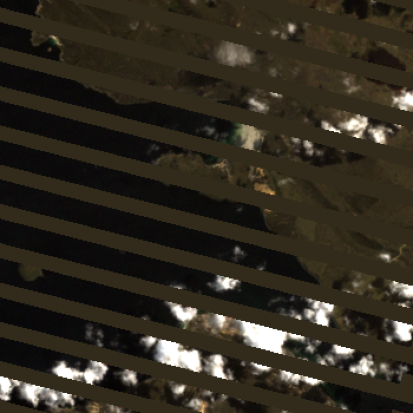
\includegraphics[width=\textwidth]{slc_image1.png} % Replace with your image file
      \label{fig:slc1}
  \end{subfigure}
  \hfill % Adds horizontal space, pushing subfigures apart if needed
  \begin{subfigure}[b]{0.3\textwidth}
      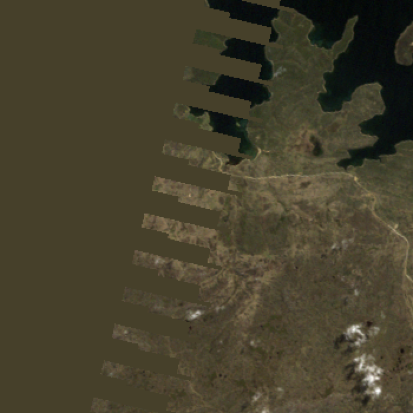
\includegraphics[width=\textwidth]{slc_image2.png} % Replace with your image file
      \label{fig:slc2}
  \end{subfigure}
  \hfill % Adds horizontal space
  \begin{subfigure}[b]{0.3\textwidth}
      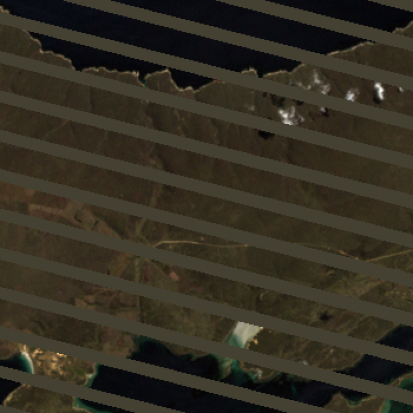
\includegraphics[width=\textwidth]{slc_image3.png} % Replace with your image file
      \label{fig:slc3}
  \end{subfigure}
  \caption{Examples of Landsat 7 SLC-off imagery illustrating the characteristic wedge-shaped data gaps caused by the Scan Line Corrector failure.}
  \label{fig:slc_failure_examples}
\end{figure}


\subsection{Established Automated Methods: Multiple Endmember Spectral Mixture Analysis} 

A prominent automated method for analyzing kelp in Landsat imagery is Multiple Endmember Spectral Mixture Analysis (MESMA). This technique models each pixel's light signature as a mix of pure reference spectra called 'endmembers,' such as 'kelp' and 'water.' A key challenge in applying Spectral Mixture Analysis to coastal environments is the high spectral variability of water. Its appearance can vary dramatically due to factors like depth, sediment load, or surface reflections, meaning it cannot be adequately represented by a single endmember. MESMA addresses this by using multiple water endmembers, often automatically extracted from pre-defined, consistently water-covered locations within each scene to create a scene-specific library (Bell et al., 2020).
    
MESMA's strength lies in providing quantitative sub-pixel fractional cover estimates, which can be linked to biomass and are suitable for large-scale automated analysis (Bell et al., 2020). However, its accuracy hinges on how well the chosen endmembers represent the actual materials. The automated selection of water endmembers from fixed points might not always capture the full spectral diversity of water in a scene or could be affected by localized noise like haze. Additionally, MESMA is known to have difficulty accurately quantifying very low kelp cover, typically below 20\% (Hamilton et al., 2020; Cavanaugh et al., 2023).

\subsection{A New Approach with an Alternative Data Source: The Floating Forests Project} 

In this project, volunteers visually inspected Landsat 7 images, which were displayed using a combination of Short-Wave Infrared (SWIR), Near-Infrared (NIR), and Red bands to enhance kelp visibility, and then manually traced the borders of visible kelp canopy. A key aspect of Floating Forests is its consensus mechanism: the final classification for any given pixel as 'kelp' or 'not kelp' did not rely on a single individual but rather on the agreement among multiple (up to 15) untrained volunteers. For instance, a pixel might be labeled as kelp only if a certain threshold of votes (e.g., >=4, as determined by Rosenthal et al.) was reached. 
       
Importantly, the utility and accuracy of this consensus-based approach have been validated. The study by Rosenthal et al. (2018) confirmed that kelp classifications derived from this citizen science consensus achieve an accuracy (measured by the Matthews Correlation Coefficient, MCC) comparable to that of expert-derived methods, thereby establishing the dataset as a reliable source of ground truth. This methodology is fundamentally different from techniques like MESMA because it relies on human visual pattern recognition and collective judgment, rather than on spectral physics and automated endmember extraction. Consequently, Floating Forests provides a label source that may capture different types of information or exhibit different sensitivities to image noise and visual ambiguities compared to purely spectral methods.

\subsection{Deep Learning for Image Segmentation} 

We employ semantic segmentation, a computer vision technique whose objective is to assign a class label to every single pixel in an image. In the context of this research, this means each pixel in a Landsat 7 image tile will be classified as either 'kelp' or 'background' (e.g., water, land, cloud). A prominent and highly effective deep learning architecture for semantic segmentation, particularly in biomedical and increasingly in remote sensing applications, is the UNet. The UNet is a type of Convolutional Neural Network (CNN) characterized by its distinctive encoder-decoder structure. The encoder part progressively downsamples the input image to capture contextual information and learn abstract features, while the decoder part gradually upsamples these features to reconstruct a full-resolution segmentation map. A key innovation of the UNet is its use of skip connections. In a standard CNN, information typically flows sequentially from one layer to its immediate neighbor. Skip connections, however, create direct pathways that allow information from earlier, higher-resolution layers in the encoder to be combined with the upsampled features in the decoder. This fusion of coarse, contextual information (from deeper layers) with fine-grained, localization-specific details (from shallower layers) enables the UNet to produce highly precise segmentations.

\subsection{Leveraging Prior Knowledge with Transfer Learning and Fine-Tuning} 

Training deep learning models like the UNet from scratch often requires vast amounts of labeled data, which can be a significant bottleneck for specialized applications. To mitigate this, our approach incorporates transfer learning. This technique involves utilizing a model, or a component of it (in our case, the encoder part of the UNet), that has already been pre-trained on a large, general-purpose dataset. For this study, we leverage ResNet architectures (such as ResNet-18, ResNet-34, or ResNet-50) that have been pre-trained on ImageNet, a massive dataset containing millions of diverse everyday images. The core idea is that these pre-trained models have already learned to recognize a rich hierarchy of visual features—from simple edges and textures to more complex object parts—which are often transferable and beneficial even for very different image domains like satellite imagery. By starting with these powerful, pre-learned features, the need for extensive labeled data specific to kelp detection is significantly reduced, and the model can often converge faster and achieve better performance.

Building upon transfer learning, we also employ fine-tuning. While the pre-trained weights provide a strong starting point, fine-tuning allows these weights within the encoder to be further updated and adjusted during the training process using our specific kelp dataset. This adaptation enables the model to refine its learned features and specialize more precisely to the unique visual characteristics, spectral signatures, and subtle patterns associated with kelp as observed in Landsat 7 satellite imagery from orbit. This process ensures that the general features learned from ImageNet are tailored to the specific nuances of the target task.

\subsection{Data Augmentation} 

Deep learning models typically perform better and generalize more effectively when trained on large and diverse datasets. However, acquiring extensive labeled data for specialized tasks can be challenging. Without sufficient data diversity, models may struggle to learn the full range of variations present in real-world scenarios, potentially leading to poor performance on unseen data and a tendency to "memorize" the limited training examples—a problem known as overfitting. Data augmentation involves artificially expanding the training dataset by applying a series of random transformations to the existing input images and their corresponding labels. Common transformations include geometric changes like horizontal and vertical flips, random rotations, or the addition of small amounts of noise. While these modifications might seem trivial to a human observer, to the model, each transformed image is perceived as a new, distinct training example. This supplemental training data created through augmentation significantly improves the model's robustness by exposing it to a wider variety of visual conditions. It enhances the model's ability to generalize to new, previously unseen images and plays a vital role in preventing overfitting.


% Start of content from Section 3 onwards

\section{Methods}

\subsection{Introduction}

The methodology involved several key stages: data acquisition and preprocessing from the Floating Forests dataset, model architecture design based on a UNet with a ResNet backbone, a training procedure incorporating data augmentation and learning rate scheduling, determination of an optimal prediction threshold, and finally, evaluation on an unseen test set.

\subsection{Data Acquisition and Description: The Floating Forests Dataset}

The primary dataset utilized for training, validating, and testing the deep learning models in this study was sourced from the Floating Forests project. This dataset consists of paired satellite imagery (features) and corresponding kelp segmentation masks (labels). The feature data comprised image tiles derived from the Landsat satellite missions. These were provided as 350 x 350 pixel, unreferenced GeoTIFF tiles, each corresponding to coastal water regions around the Falkland Islands. Each GeoTIFF image tile contained seven co-referenced data bands, all at a 30-meter spatial resolution:

\begin{itemize}
    \item \textbf{Bands 0-4 (Spectral Bands):} These five bands represent surface reflectance data and were rescaled to 16-bit integers. They include, in order: Short-Wave Infrared 1 (SWIR1), Near-Infrared (NIR), Red, Green, and Blue. A pixel value of -32768 within these bands indicated missing data.
    \item \textbf{Band 5 (Cloud Mask):} This was a binary mask where a value of 1 signified the presence of a cloud, and 0 indicated no cloud, serving as a critical quality layer.
    \item \textbf{Band 6 (Digital Elevation Model - DEM):} This band provided elevation data in meters above sea level, primarily derived from ASTER (Advanced Spaceborne Thermal Emission and Reflection Radiometer) data.
\end{itemize}
The satellite image tiles followed a consistent filename schema: \texttt{<tile\_id>\_satellite.tif}.

The corresponding label data consisted of binary segmentation masks, with pixel values indicating the presence (1) or absence (0) of kelp canopy. These ground truth masks were generated by citizen scientists participating in the Floating Forests study. These masks were provided as single-band, 350 x 350 pixel TIFF images, matching the dimensions of the feature data, and used the filename schema: \texttt{<tile\_id>\_kelp.tif}.

The original Floating Forests data source provided a 'train' set, containing both feature images and their corresponding kelp labels, and a 'test' set, which included only feature images (with labels withheld by the project organizers). For the purposes of this study, the provided 'train' set was further subdivided to create our own distinct training, validation, and test partitions to ensure rigorous model development and evaluation.

\subsection{Data Preprocessing and Cleaning}

The cleaning process began by identifying and flagging invalid or unusable pixels within each image tile. Pixels were marked as invalid if they contained the specific no-data marker value of -32768, a standard indicator of missing data in the original Landsat processing, or if they had negative values in any of the primary spectral bands (Bands 0-4). Concurrently, pixels corresponding to clouds were identified using the provided cloud mask (Band 5), and pixels representing land were identified using the Digital Elevation Model (DEM, Band 6), specifically where DEM values were greater than 0 meters.

Once invalid pixels (no-data markers, negative values), clouds, and land areas were identified, the next step involved addressing potential extreme outliers in the spectral bands (Bands 0-4) and the DEM band (Band 6). Prior to calculating the statistics needed for normalization, pixel values in these target bands were clipped based on pre-defined global thresholds. These thresholds, corresponding to the approximate 1st and 99th percentiles of the data distribution for each band, were determined from an initial exploratory analysis of the entire dataset. This clipping step served to mitigate the influence of extreme, potentially erroneous pixel values on the subsequent calculation of normalization parameters. 

\begin{figure}[htbp]
    \centering
    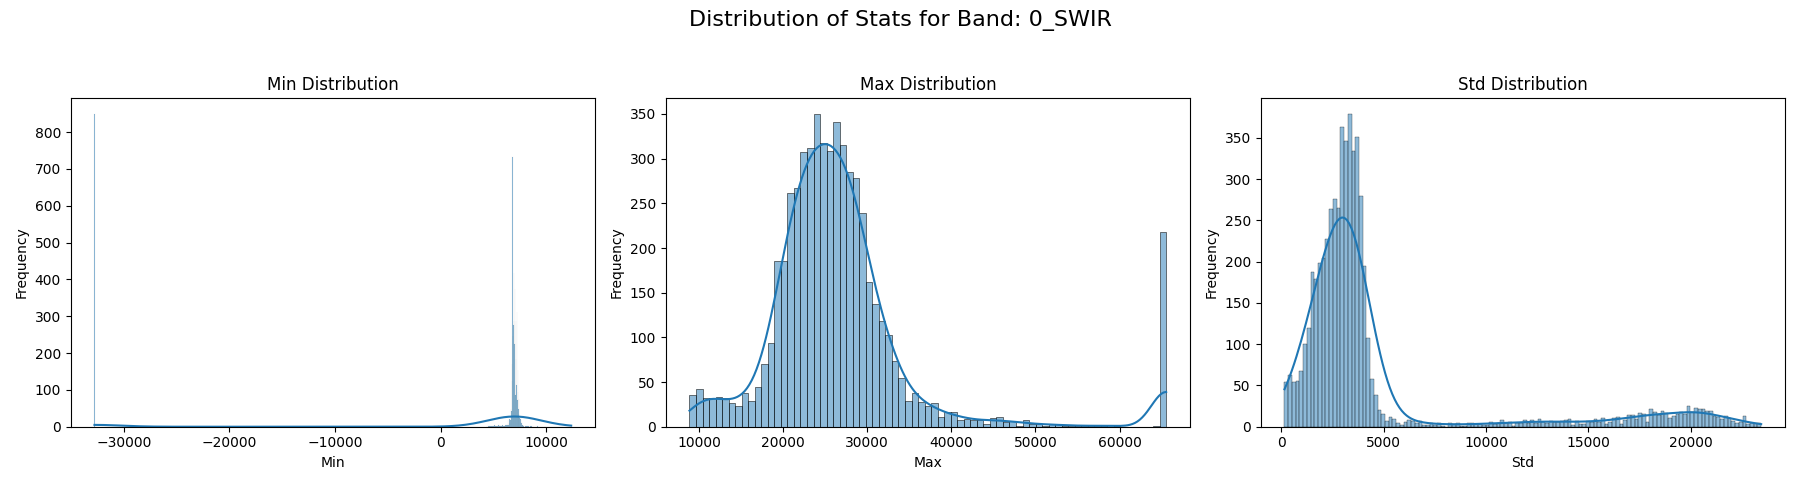
\includegraphics[width=\textwidth]{distribution_0_SWIR_before.png} % REPLACE WITH YOUR 'BEFORE' IMAGE FILENAME
    \caption{Distribution of pixel value statistics (Min, Max, Std) for Band 0 (SWIR) across the dataset \textit{before} outlier clipping and normalization, illustrating the presence of extreme values.}
    \label{fig:stats_before}
\end{figure}

Following this outlier treatment, dataset-wide mean and standard deviation were calculated for each of the clipped spectral bands (Bands 0-4) and the clipped DEM band (Band 6). Critically, the pixels flagged in the initial identification step (no-data markers, negative values, clouds, and land) were still excluded from these statistical calculations to ensure that the derived means and standard deviations were representative of valid, clipped water and potential kelp pixels only.

Following clipping and normalization, Z-score standardization was applied, where each pixel value in the spectral bands (0-4) and the DEM band (6) was transformed by subtracting the previously calculated mean for that band and then dividing by its standard deviation. After this standardization, any pixels that were originally identified as invalid due to the -32768 marker or negative reflectance values were replaced with a value of 0.0, as 0.0 represents the mean of a Z-score standardized distribution and thus minimizes the impact of these values on subsequent model layers. The original binary cloud mask (Band 5) was preserved throughout this process without any numerical normalization or clipping. Finally, the processed images, now containing the normalized spectral and DEM bands alongside the original cloud mask, were saved back in-place as 32-bit floating-point TIFF files, maintaining the (Height, Width, Channels) format. 

\begin{figure}[htbp]
    \centering
    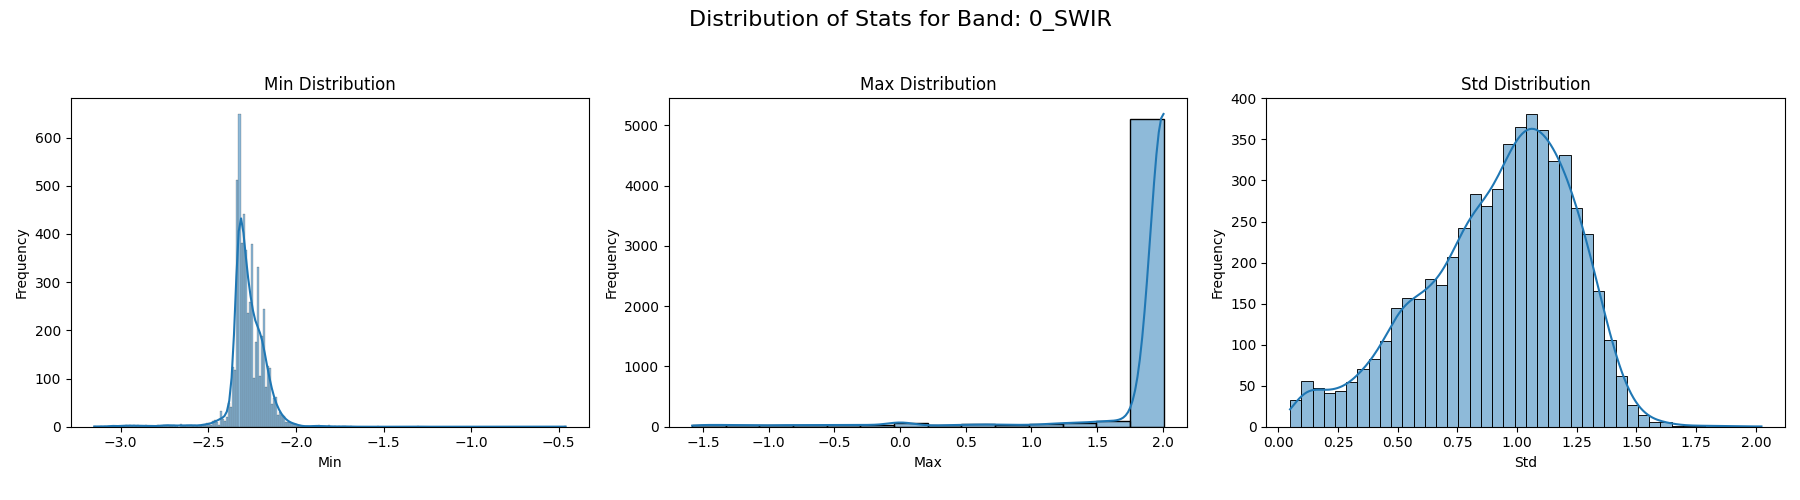
\includegraphics[width=\textwidth]{distribution_0_SWIR_after.png} % REPLACE WITH YOUR 'AFTER' IMAGE FILENAME
    \caption{Distribution of pixel value statistics (Min, Max, Std) for Band 0 (SWIR) across the dataset \textit{after} outlier clipping and Z-score normalization, showing a more concentrated and standardized distribution.}
    \label{fig:stats_after}
\end{figure}

\subsection{Dataset Splitting}

Following the initial data acquisition and preprocessing, the complete set of 5,635 paired satellite image tiles and their corresponding ground truth kelp masks (derived from the original Floating Forests 'train' set) was systematically divided into three distinct subsets: training, validation, and test. This partitioning was achieved by running a dedicated script that randomly assigned images to ensure an approximate 70\%, 15\%, and 15\% split, respectively. The resulting 'train' set was used exclusively for training the deep learning model. The 'validation' set was used during the training process for monitoring model performance after each epoch and was also later utilized to determine the optimal probability threshold for classifying pixels as kelp. Finally, the 'test' set was strictly held out and remained unseen by the model until the final evaluation phase, serving as a true measure of the model's generalization capabilities on previously unencountered data. This splitting procedure resulted in the creation of six distinct folders: a satellite image folder and a ground truth mask folder for each of the training, validation, and test sets.

\subsection{Model Development and Training}

This section details the architecture of the deep learning model employed for kelp segmentation, the data handling procedures, and the comprehensive training setup.

\subsubsection{Model Architecture}

A U-Net-like semantic segmentation model formed the core of our approach, utilizing a pre-trained ResNet architecture as its encoder backbone. The specific ResNet variant (ResNet18, ResNet34, or ResNet50) was configurable, allowing for experimentation with different model capacities. The UNet architecture was selected due to its well-documented effectiveness in biomedical image segmentation and its increasing adoption and success in remote sensing applications. Its characteristic encoder-decoder structure, augmented with skip connections, is adept at capturing both broad contextual information and precise local features, making it highly suitable for pixel-wise segmentation tasks like delineating kelp canopy. 

To adapt the pre-trained ResNet encoder to our specific 7-channel satellite imagery, its initial convolutional layer was modified to accept seven input channels instead of the standard three (RGB). The decoder component of the UNet was custom-built, composed of sequential blocks of 2D transposed convolution for upsampling, followed by Batch Normalization and Rectified Linear Unit activation layers. This decoder comprised four such upsampling blocks, designed to progressively increase the spatial resolution of the feature maps while reducing their channel depth. Starting from the encoder's output (which has 512 channels for ResNet18/34 or 2048 for ResNet50), the decoder passed features through intermediate channel depths of 256, 128, and 64, eventually down to 32 channels. A final 1x1 convolutional layer then transformed these features into a single-channel output representing the raw logits for binary (kelp/no-kelp) segmentation.

\subsubsection{Data Handling and Augmentation}

During training, the input satellite image tiles were subjected to on-the-fly data augmentation to artificially increase the diversity of the training set and improve model robustness. The augmentations applied included horizontal flips, vertical flips, random 90-degree rotations, and the addition of small amounts of Gaussian noise to the primary spectral bands (Bands 0-4). Each of these transformations had a 50\% probability of being applied to any given training image. In contrast, the validation data was not augmented to ensure an unbiased evaluation of the model's performance at each epoch. Data for both training and validation was loaded using PyTorch DataLoaders, with a batch size of 8 for training and 16 for validation.

\subsubsection{Training Setup and Procedure}

The model training process used the PyTorch Lightning framework, which streamlines deep learning experimentation. The loss function chosen for optimizing the model was Binary Cross-Entropy with Logits (BCEWithLogitsLoss), suitable for binary pixel-wise classification tasks. During each validation step, the Intersection over Union (IoU) for the ``kelp'' class was calculated and logged. IoU, also known as the Jaccard Index, was selected as the primary evaluation metric because it is a standard and robust measure for assessing the accuracy of semantic segmentation models, quantifying the overlap between predicted and ground truth regions.

The Adam optimizer was employed for updating model weights, initialized with a learning rate of 1e-4. Adam (Adaptive Moment Estimation) is a widely used optimization algorithm that combines the advantages of AdaGrad (which adapts learning rates per parameter) and RMSProp (which uses a moving average of squared gradients), often leading to efficient convergence and good performance across various deep learning tasks. To manage the learning rate throughout training, a Cosine Annealing learning rate scheduler (CosineAnnealingLR) was utilized. This scheduler gradually reduced the learning rate over a maximum of 400 epochs down to a minimum value of 1e-7. A custom LearningRateMonitor callback was implemented to log and print these learning rate changes.

Training was configured to run for a maximum of 400 epochs, but an EarlyStopping callback was also implemented to prevent overfitting and save computational resources. This callback monitored the validation loss and would halt training if the loss did not improve by at least a minimum delta of 0.001 for 100 consecutive epochs. Furthermore, a Model Checkpoint callback automatically saved the model checkpoint that achieved the best validation loss observed during the entire training run. The training script also included functionality to resume training from the latest available checkpoint if a previous run within the same output directory was interrupted.

\subsubsection{Hardware, Precision, and Final Model Output}

Training was conducted utilizing GPU acceleration when available, with experiments run on NVIDIA GTX 1060 3GB and GTX 1080 Ti 11GB graphics cards. For all GPU-based training, 32-bit floating-point precision was specified. Upon completion of the training process (either by reaching the maximum number of epochs or due to early stopping), the state dictionary of the model that achieved the best validation loss throughout the entire training run was saved as a .pth file. This file represents the finalized, trained model weights ready for inference and evaluation.

\subsection{Determining the Optimal Prediction Threshold}

The output of the trained semantic segmentation model for each pixel is a continuous probability score, representing the model's confidence that the pixel belongs to the 'kelp' class. To convert these probabilistic outputs into definitive binary predictions for practical application and quantitative evaluation, a specific probability threshold must be established. A dedicated script was therefore employed to determine the optimal threshold. This script first loaded the best performing model weights saved from a completed training run. The model was applied to all images in the validation set to generate raw sigmoid output probabilities for every pixel. Then, a predefined range of potential threshold values, from 0.2 to 0.6 iterated in steps of 0.004, was systematically tested. For each candidate threshold in this range, the pre-computed probabilities from the validation set were converted into binary segmentation masks. The Intersection over Union (IoU) score was calculated for each set of resulting binary masks against the ground truth validation labels. The threshold value that yielded the maximum IoU score on this validation set was then selected and designated as the optimal prediction threshold for that specific model and training run.

\subsection{Model Evaluation on the Test Set}

To assess the generalization performance of the trained segmentation model on entirely unseen data, a dedicated evaluation script was utilized. The evaluation was performed on the held-out test dataset, which consisted of satellite images and their corresponding ground truth kelp masks from the pre-defined test split directories. During inference, the model processed each image in the test set, generating raw sigmoid probability outputs for every pixel. These probabilities were then converted into binary (kelp/no-kelp) predictions using the pre-determined optimal threshold. 

An optional land mask post-processing step was available: if enabled, this step would reclassify any pixels predicted as kelp that corresponded to land areas to 'no-kelp', ensuring predictions were confined to water bodies. Following this post-processing, the performance of the model was quantified by calculating four standard segmentation metrics, comparing the final binary predictions against the ground truth test masks: IoU, Precision, Recall, and the F1-Score. Finally, the resulting binary prediction masks for the test set were saved as TIFF files for qualitative review and archival.

\section{Results}

\subsection{Overview of Experimental Setup} % Note: Expiramental corrected to Experimental

This section presents the quantitative outcomes of the experiments conducted to evaluate the performance of the developed deep learning pipeline for kelp canopy segmentation. The primary experimental variables investigated included the effect of data preprocessing, the impact of applying random data augmentation techniques during training, and a comparative analysis of model performance across different ResNet encoder backbones (specifically ResNet18, ResNet34, and ResNet50). Additionally, the influence of a land mask post-processing step, designed to correct potential misclassifications of kelp over land areas, was evaluated. For all experimental configurations, model performance was assessed using four standard segmentation metrics— IoU, Precision, Recall, and the F1-Score calculated on the held-out test set to ensure an unbiased measure of generalization capability.

\subsection{Impact of Data Preprocessing}

\begin{table}[htbp] % Figure placement options: h=here, t=top, b=bottom, p=page of floats
  \caption{Impact of Data Preprocessing (Cleaning) on Model Performance. All models trained without data augmentation.}
  \label{table:preprocessing_impact}
  \centering
  \begin{tabular}{lllllll}
    \toprule
    Backbone & Preprocessing & Augmentation & IoU    & Precision & Recall & F1-Score \\
    \midrule
    ResNet18 & Original      & No           & 0.3043 & 0.4192    & 0.5261 & 0.4666   \\
    ResNet18 & Cleaned       & No           & 0.4437 & 0.5874    & 0.6446 & 0.6147   \\
    ResNet34 & Original      & No           & 0.3239 & 0.4645    & 0.5168 & 0.4893   \\
    ResNet34 & Cleaned       & No           & 0.4492 & 0.5827    & 0.6622 & 0.6200   \\
    ResNet50 & Original      & No           & 0.3656 & 0.5178    & 0.5543 & 0.5354   \\
    ResNet50 & Cleaned       & No           & 0.4419 & 0.5782    & 0.6521 & 0.6130   \\
    \bottomrule
  \end{tabular}
\end{table}

The application of data cleaning and normalization procedures consistently improved model performance across all ResNet backbones when augmentations were not used. For instance, with the ResNet18 backbone, IoU increased from 0.3043 (original data) to 0.4437 (cleaned data), representing a substantial improvement of 45\%. Similarly, ResNet34 saw an improvement of 38\%, and ResNet50 saw 20\%. Data cleaning was a crucial step for achieving better baseline performance.

\subsection{Impact of Data Augmentation} % Assuming this was meant to be 4.3, renumbering for consistency. If 4.3 was different, please let me know.

\begin{table}[htbp] % Figure placement options: h=here, t=top, b=bottom, p=page of floats
  \caption{Impact of Data Augmentation on Model Performance. All models trained with cleaned data.}
  \label{table:augmentation_impact}
  \centering
  \begin{tabular}{lllllll}
    \toprule
    Backbone & Preprocessing & Augmentation & IoU    & Precision & Recall & F1-Score \\
    \midrule
    ResNet18 & Cleaned       & No           & 0.4437 & 0.5874    & 0.6446 & 0.6147   \\
    ResNet18 & Cleaned       & Yes          & 0.4983 & 0.6387    & 0.6939 & 0.6652   \\
    ResNet34 & Cleaned       & No           & 0.4492 & 0.5827    & 0.6622 & 0.6200   \\
    ResNet34 & Cleaned       & Yes          & 0.5028 & 0.6355    & 0.7066 & 0.6692   \\
    ResNet50 & Cleaned       & No           & 0.4419 & 0.5782    & 0.6521 & 0.6130   \\
    ResNet50 & Cleaned       & Yes          & 0.5010 & 0.6386    & 0.6993 & 0.6676   \\
    \bottomrule
  \end{tabular}
\end{table}

Data augmentation applied during training on the cleaned dataset further enhanced model performance for all backbones. With the ResNet18 backbone, IoU improved from 0.4437 (no augmentation) to 0.4983 (with augmentation). The ResNet34 backbone showed the highest overall performance when combined with cleaned data and augmentations, achieving an IoU of 0.5028 and an F1-Score of 0.6692. ResNet50 saw a very similar increase in performance. Data augmentation provided a significant boost to the models trained on cleaned data.

\newpage

\subsection{Comparison of ResNet Backbones} % Renumbering from 4.5

\begin{table}[htbp] % Figure placement options: h=here, t=top, b=bottom, p=page of floats
  \caption{Comparison of ResNet Backbones. All models trained with cleaned data and data augmentation.}
  \label{table:backbone_comparison}
  \centering
  \begin{tabular}{lllllll}
    \toprule
    Backbone & Preprocessing & Augmentation & IoU    & Precision & Recall & F1-Score \\
    \midrule
    ResNet18 & Cleaned       & Yes          & 0.4983 & 0.6387    & 0.6939 & 0.6652   \\
    ResNet34 & Cleaned       & Yes          & 0.5028 & 0.6355    & 0.7066 & 0.6692   \\
    ResNet50 & Cleaned       & Yes          & 0.5010 & 0.6386    & 0.6993 & 0.6676   \\
    \bottomrule
  \end{tabular}
\end{table}

When comparing the performance of different ResNet backbones using cleaned data and augmentations, the ResNet34 backbone achieved the highest IoU (0.5028) and F1-Score (0.6692). The ResNet50 backbone performed comparably (IoU: 0.5010, F1: 0.6676), while the ResNet18 backbone was slightly lower (IoU: 0.4983, F1: 0.6652). This suggests that while deeper models offered a slight advantage, the gains diminished beyond ResNet34 for this specific task and dataset.

\subsection{Effect of Land Mask Post-processing} % Renumbering from 4.6

The impact of applying a land mask as a post-processing step—designed to eliminate any kelp predictions occurring over land areas (identified by DEM values > 0)— was evaluated. Across the vast majority of experimental conditions, encompassing different ResNet backbones, data preprocessing strategies, and the application of data augmentation, this land mask post-processing step had a negligible or no discernible impact on the primary evaluation metrics. For instance, the best-performing model configuration (UNet with a ResNet34 backbone, trained on cleaned data with augmentations) achieved an IoU of 0.5028 both with and without the application of the land mask. While minor variations were observed in some lower-performing, less optimized model runs, this effect was not apparent in the higher-performing models. This suggests that for the primary test set evaluations, the better-trained models were largely not predicting significant amounts of kelp over land areas, or if such misclassifications occurred, they did not substantially affect the overall segmentation performance metrics for kelp itself.

\subsection{Summary of Best Performing Model} % Renumbering from 4.7

The best overall performance was achieved using a UNet with a ResNet34 backbone, trained on cleaned and normalized data with data augmentations applied. This configuration yielded an Intersection over Union (IoU) of 0.5028, a Precision of 0.6355, a Recall of 0.7066, and an F1-Score of 0.6692 on the held-out test set, using a prediction threshold of 0.3414.

\newpage

\subsection{Qualitative Results} % Renumbering from 4.8

To visually assess the model's performance, representative examples of predictions from the best-performing model (ResNet34, cleaned, augmented) on test set images are presented below.

\begin{figure}[htbp]
    \centering
    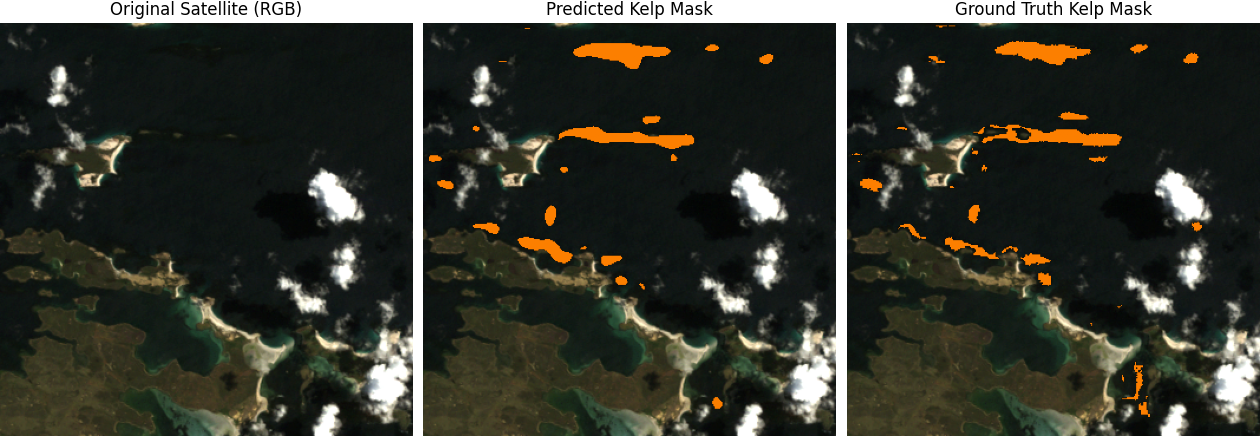
\includegraphics[width=0.8\textwidth]{good2.png} % Adjust width as needed
    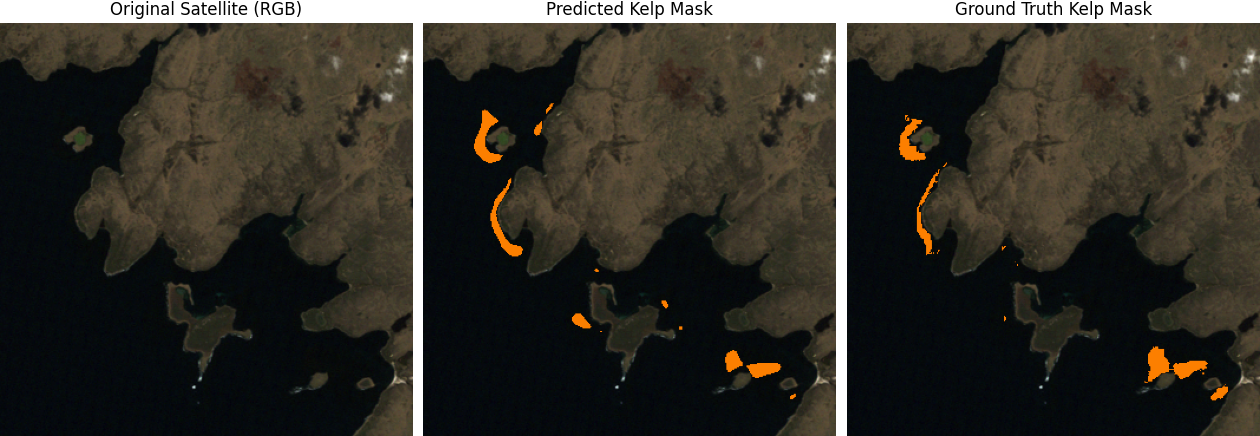
\includegraphics[width=0.8\textwidth]{good3.png}
    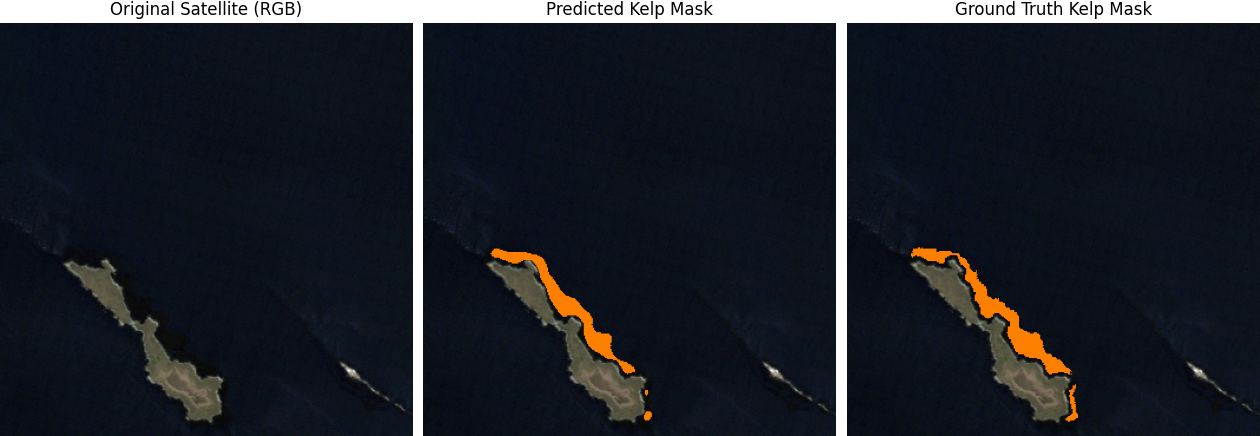
\includegraphics[width=0.8\textwidth]{good1.png}
    \caption{Successful segmentation of clear kelp patches. These examples illustrate the model's ability to accurately delineate well-defined kelp canopy under favorable conditions.}
    \label{fig:good_segmentation}
\end{figure}

\begin{figure}[htbp]
    \centering
    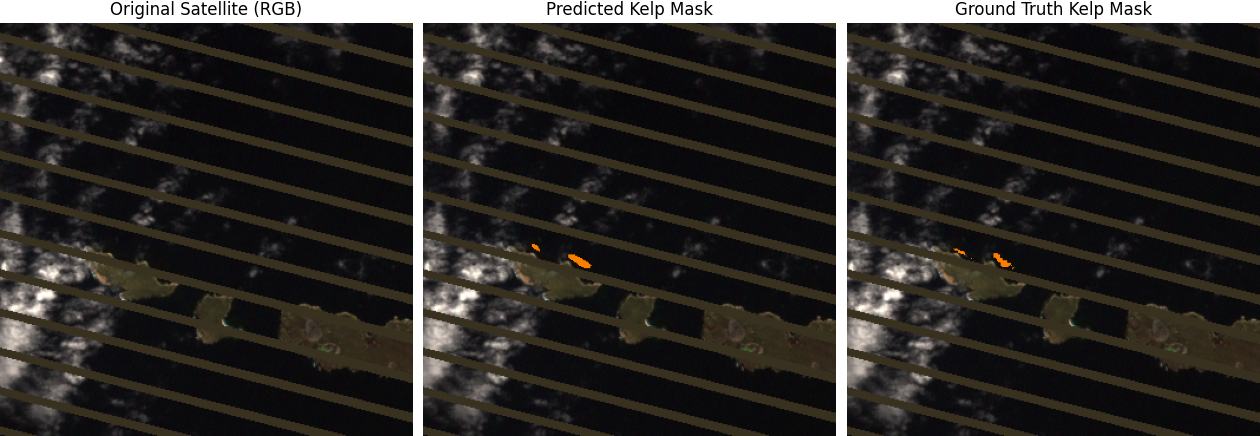
\includegraphics[width=0.8\textwidth]{goodslc.png} % Adjust width as needed
    \caption{Example of model performance on an image affected by Landsat 7 SLC-off data gaps. Even with missing data strips, the model demonstrates an ability to identify kelp in the visible portions.}
    \label{fig:slc_performance}
\end{figure}

\begin{figure}[htbp]
    \centering
    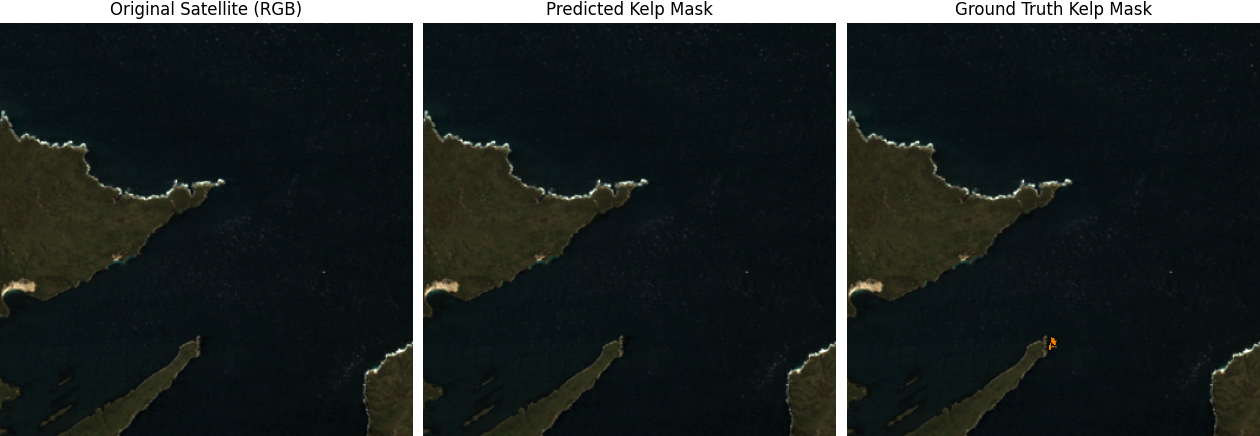
\includegraphics[width=0.8\textwidth]{bad1.png} % Adjust width as needed
    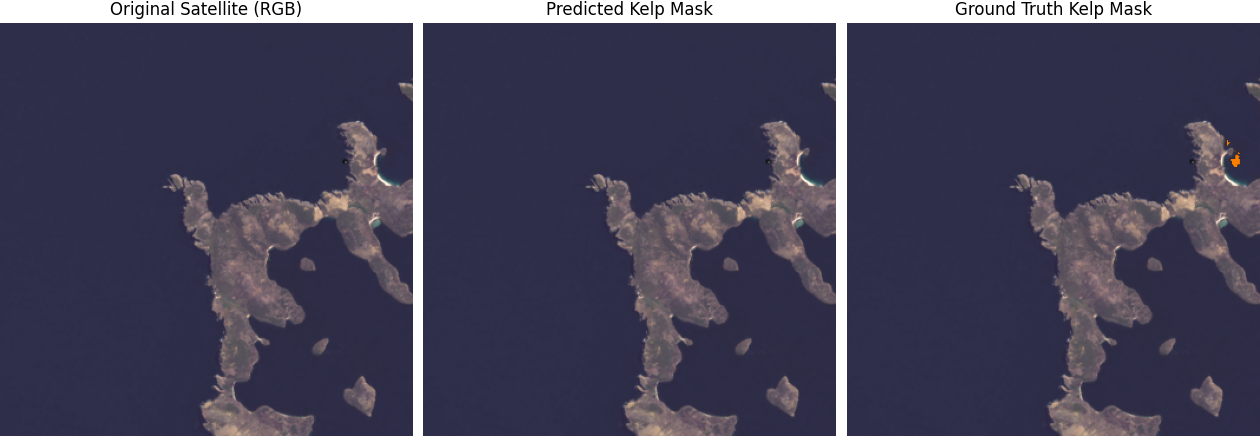
\includegraphics[width=0.8\textwidth]{bad2.png}
    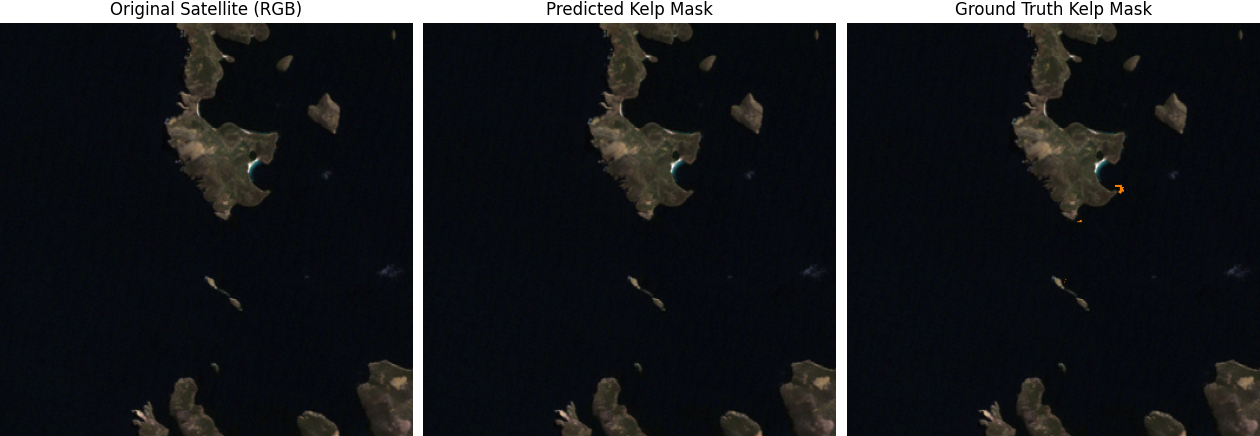
\includegraphics[width=0.8\textwidth]{bad3.png}
    \caption{Examples of poor performance and missed detections, particularly for small or sparse patches of kelp. These highlight instances where the model struggled, potentially due to the 30m resolution limit or less distinct kelp signatures.}
    \label{fig:poor_segmentation}
\end{figure}


\section{Discussion}

\subsection{Summary of Key Findings and Performance}

This study successfully demonstrated the development and viability of an end-to-end deep learning pipeline, specifically a UNet architecture with a ResNet encoder, for the automated segmentation of kelp canopy using Landsat 7 imagery and ground truth labels derived from the Floating Forests citizen science project. The optimal configuration, employing a ResNet34 backbone trained on cleaned and augmented data, achieved a notable Intersection over Union (IoU) of 0.5028 on the held-out test set. Key to achieving this level of performance were the rigorous data preprocessing steps, including cleaning and normalization, and the strategic use of data augmentation. Furthermore, initial explorations underscored the critical importance of transfer learning; attempts to train models from scratch proved infeasible with the available labeled data, making the use of pre-trained encoder weights followed by fine-tuning an essential component for generating accurate kelp masks. Finally, the application of a land mask post-processing step had a negligible impact on the performance of the best models, suggesting a good degree of specificity in distinguishing kelp from land areas.

\subsection{Interpretation of Results: Factors Contributing to Model Success}

The successful performance of the deep learning pipeline can be attributed to several key methodological choices and data characteristics, each playing a vital role in enabling the model to effectively learn and segment kelp canopy.

\subsubsection{The Importance of Data Preprocessing: Stabilizing Input Distributions}

The data cleaning and normalization process was fundamental to achieving robust model performance. Z-score standardization rescaled input features to a common range (zero mean, unit variance), which stabilizes the learning process by preventing features with larger numerical values from disproportionately influencing model weight updates, thereby promoting faster and more stable convergence. Pre-normalization clipping of extreme values further reduced the impact of sensor artifacts or rare environmental conditions that could skew the data distribution. Additionally, handling no-data markers (-32768) and meaningless negative values by replacing them with a neutral value (0.0 post-standardization) ensured these pixels did not introduce disruptive NaNs or extreme values into calculations. These steps significantly reduced noise inherent in satellite imagery—stemming from sensor imperfections, atmospheric interference, or bi-directional reflectance effects—allowing the model to focus on learning meaningful underlying features indicative of kelp rather than spurious artifacts.

\subsubsection{The Power of Data Augmentation: Enhancing Generalization}

Data augmentation proved to be a critical strategy for improving model generalization and preventing overfitting, especially given the finite size of the training dataset. By applying random transformations such as flips, rotations, and minor noise injection, the training dataset was artificially expanded, exposing the model to a wider range of visual variations without requiring additional manually labeled data. This forced the model to learn features invariant to such transformations, enhancing its ability to generalize to unseen test data which might exhibit similar variations in kelp orientation or minor sensor noise. 

\subsubsection{The Essential Role of Transfer Learning and Fine-Tuning}

The adoption of transfer learning, utilizing ResNet backbones pre-trained on the large and diverse ImageNet dataset, was essential for the project's success. These pre-trained models have already learned a rich hierarchy of visual features (edges, textures, shapes) in their early and mid-level layers, many of which are transferable to the domain of satellite imagery analysis. Attempting to train a deep network of this complexity from scratch on the relatively small Floating Forests dataset would likely have been infeasible, requiring vastly more labeled examples to learn meaningful representations. Starting with pre-trained weights provided a much stronger initialization, enabling faster convergence to a more effective solution. Subsequent fine-tuning allowed these pre-learned general features to be adapted and specialized to the specific visual nuances and spectral patterns of kelp as observed in Landsat 7 imagery, ensuring the model was tailored to the target task.

\subsubsection{Backbone Choice: ResNet34 as an Effective Compromise}

The experimental results indicated that the ResNet34 backbone offered a favorable balance of model capacity and performance for this specific task. It likely possessed sufficient depth and parameters to learn the complex features required to distinguish kelp in 30m resolution Landsat imagery using the Floating Forests labels. While the deeper ResNet50 model is theoretically more powerful, the marginal, if any, performance gains observed suggested that its additional complexity might have increased the risk of overfitting to the available training data without providing a significant advantage in discriminative power for this particular problem. Conversely, ResNet18, though still effective due to transfer learning, may have had slightly insufficient capacity to capture all the necessary distinguishing features compared to ResNet34.

\subsubsection{Strategic Thresholding for Optimal Binary Classification}

The final step of converting the model's probabilistic outputs to binary classifications relied on selecting an optimal threshold. This threshold was determined by maximizing the IoU score on the validation set, ensuring that the binary predictions aligned as closely as possible with the ground truth according to this robust segmentation metric. The observation that optimal thresholds varied between different experimental runs underscores that this value is not universal; it is influenced by the specific model architecture and training data characteristics. The chosen threshold effectively balanced the trade-off between precision (minimizing false positives) and recall (minimizing false negatives) to achieve the best overall segmentation performance as measured by IoU.

\subsection{The Developed End-to-End Solution and its Significance}

This study successfully developed and demonstrated a complete, end-to-end pipeline for the automated segmentation of kelp canopy, transforming raw satellite image tiles into actionable binary prediction masks. This automated approach presents several significant advancements over traditional kelp monitoring methods. Unlike costly aerial surveys, such as those conducted by the California Department of Fish and Wildlife, this method leverages pre-existing, freely available Landsat imagery. This eliminates the substantial financial outlay and logistical complexities associated with dedicated aerial image acquisition campaigns. Furthermore, the deep learning model automates the segmentation process itself, removing the need for ongoing, time-consuming manual delineation of kelp by experts for each new satellite image—a major bottleneck that characterizes methods like the traditional CDFW aerial survey processing. 

This automated, model-based system is inherently scalable, capable of processing vast archives of satellite imagery far more rapidly than any manual method. The consistent revisit cycle of satellites like Landsat further enhances its utility by enabling the tracking of changes in kelp extent over time, which is crucial for identifying areas undergoing ecological stress. Perhaps most critically, by reducing the expenditure typically required for image acquisition and manual annotation, the resources saved can be reallocated to more direct and impactful conservation efforts. Specifically, these financial savings could be channeled towards funding more diver-based interventions, such as targeted urchin removal in areas identified by the model as having declining kelp cover or being otherwise at risk. Therefore, the developed solution can contribute to a more cost-effective, responsive, and efficient cycle of kelp forest monitoring and management, enabling a more strategic allocation of limited conservation funds to where they are most needed on the seafloor.

\subsection{Comparison with Existing Remote Sensing Methods}

The deep learning pipeline developed in this study offers a distinct alternative to existing remote sensing methods for kelp mapping. When compared to established automated techniques like MESMA (Bell et al., 2020), which provides valuable fractional cover estimates, our approach differs fundamentally. MESMA relies on spectral unmixing and pre-defined or scene-specific endmembers, whereas our model, trained on human-consensus labels from Floating Forests, learns to identify kelp based on spatial patterns and visual cues directly from the imagery. This difference presents potential advantages: our deep learning model might exhibit different robustness characteristics to certain atmospheric or water conditions if key visual patterns remain discernible, and once trained, it does not require per-scene endmember refinement. Furthermore, because the Floating Forests dataset included SLC-off imagery, our model demonstrated an ability to produce segmentations even on this corrupted data. However, a current disadvantage is that our model produces a binary (presence/absence) output rather than the quantitative fractional cover offered by MESMA, and its performance is inherently tied to the quality and characteristics of the Floating Forests labels.

In relation to the Floating Forests project itself, which provides validated labels (Rosenthal et al., 2018), our work serves as an extension and automation of its utility. While Floating Forests provides a crucial historical dataset of kelp classifications, our deep learning pipeline leverages this past citizen science effort to build a predictive tool capable of automatically segmenting kelp in new, unseen Landsat imagery. This provides a consistent, algorithmic interpretation for ongoing monitoring, rather than relying on continuous volunteer consensus for every new image. Compared to high-resolution methods like CDFW aerial surveys or UAV-based mapping (e.g., Saccomanno et al., 2022), our satellite-based automated pipeline offers superior scalability for consistent, large-area regional monitoring due to the systematic and broad coverage of Landsat imagery. Our approach also significantly lowers operational costs by eliminating the need for dedicated aircraft/drone flights, extensive field crew deployment, and the intensive manual image processing inherent in those higher-resolution but more logistically demanding survey methods. Finally, leveraging the regular revisit cycle of satellites like Landsat allows for potentially more frequent assessments across broad areas compared to the often intermittent survey schedules of aerial and UAV campaigns.

\subsection{Limitations of the Study}

While this study demonstrates the feasibility of automated kelp mapping using deep learning, several limitations should be acknowledged. Firstly, the model's performance is inherently linked to the quality and characteristics of the Floating Forests labels used for training. Although these citizen-science-derived consensus labels have been validated, they may still contain inherent inconsistencies or differ from delineations made by trained experts in some specific instances. Secondly, the 30-meter spatial resolution of the Landsat 7 imagery inherently limits the model's ability to detect very small or sparse patches of kelp that fall below this resolution threshold. Thirdly, the current model provides a binary (presence/absence) output for kelp, which, unlike methods such as MESMA, does not quantify sub-pixel kelp density or provide direct estimates of biomass. Furthermore, the model was trained and evaluated exclusively on data from the Falkland Islands; its generalization performance on other geographic regions—which may feature different kelp species, water conditions, or atmospheric characteristics—would require further validation and potentially retraining or fine-tuning. Finally, the current iteration of the model processes each satellite image independently and does not yet leverage temporal information from sequential satellite passes, the incorporation of which could potentially improve segmentation accuracy and consistency over time.

\subsection{Future Work and Directions}

Building upon the findings of this study, several avenues for future research and development could further enhance the capabilities and applicability of the automated kelp mapping pipeline. A natural next step would be to apply and evaluate the pipeline on imagery from more recent satellite missions like Landsat 8/9 or the Sentinel-2 constellation, which offer different spectral characteristics and, in the case of Sentinel-2, higher spatial resolution that could improve the detection of smaller kelp patches. Expanding the training dataset to include more diverse geographic regions and greater temporal coverage, potentially by incorporating additional labels from Floating Forests or other emerging data sources, would be crucial for improving model generalization across different environments. 

\subsection{Broader Implications and Conclusion}

In conclusion, this research successfully demonstrates the development and operational viability of an automated, end-to-end deep learning pipeline capable of segmenting kelp canopy from satellite imagery, effectively transforming raw image inputs into map outputs. A key highlight of this study is the powerful synergy achieved by integrating large-scale, human-generated labels from citizen science initiatives like Floating Forests with the sophisticated pattern recognition capabilities of modern deep learning techniques. This combination not only validates the immense value of crowdsourced efforts in scientific research but also provides a robust foundation for training complex models. Ultimately, the approach presented here holds significant potential to enhance the efficiency, scalability, and cost-effectiveness of kelp forest monitoring. By reducing reliance on expensive and time-consuming manual methods, this technology can support more timely and targeted conservation and restoration strategies. The continued refinement and adoption of such automated systems are therefore encouraged, as they can free up critical resources, enabling their reallocation towards direct, on-the-ground interventions like urchin removal, which are essential for the recovery and long-term health of these vital coastal ecosystems. This work serves as a compelling example of how innovative computational tools, fueled by community engagement, can contribute meaningfully to addressing pressing environmental challenges.

% End of content
\newpage

\section*{}
\begingroup % Start a group to keep font size change local
\small % Optional: Reduce font size to 9 point

\begin{thebibliography}{99} % The {99} is a placeholder for the widest label, affects indentation

\bibitem{Hohman2023}
Hohman, R., Bell, T., Cavanaugh, K., Contolini, G., Elsmore, K., FloresMiller, R., Garza, C., Hewerdine, W., Iampietro, P., Nickels, A., Saccomanno, V., \& Tezak, S. (2023).
\textit{Remote sensing tools for mapping and monitoring kelp forests along the West Coast.}
National Marine Sanctuaries Conservation Series ONMS-23-10. U.S. Department of Commerce, National Oceanic and Atmospheric Administration, Office of National Marine Sanctuaries.

\bibitem{Zuckerman2023}
Zuckerman, C. (2023, May 26).
The vanishing kelp forest.
\textit{The Nature Conservancy}.
Retrieved from \url{https://www.nature.org/en-us/magazine/magazine-articles/kelp-forest/}

\bibitem{Saccomanno2022}
Saccomanno, V. R., Bell, T., Pawlak, C., Stanley, C. K., Cavanaugh, K. C., Hohman, R., Klausmeyer, K. R., Cavanaugh, K., Nickels, A., Hewerdine, W., Garza, C., Fleener, G., \& Gleason, M. (2022).
Using unoccupied aerial vehicles to map and monitor changes in emergent kelp canopy after an ecological regime shift.
\textit{Remote Sensing in Ecology and Conservation, 9}(1), 62--75.
\url{https://doi.org/10.1002/rse2.295}

\bibitem{MBC2017}
MBC Applied Environmental Sciences. (2017, August 14).
\textit{Status of the Kelp Beds in 2016: Ventura, Los Angeles, Orange, and San Diego Counties.}
Prepared for: Central Region Kelp Survey Consortium and Region Nine Kelp Survey Consortium. MBC Applied Environmental Sciences, Costa Mesa, California.

\bibitem{Bell2018_RSE} % Changed key to be more specific if you resolve year discrepancy
Bell, T. W., Cavanaugh, K. C., \& Siegel, D. A. (2020).
Three decades of variability in California's giant kelp forests from the Landsat satellites.
\textit{Remote Sensing of Environment, 218}, 26--38.
\url{https://doi.org/10.1016/j.rse.2018.06.039}
% Note: Your text cited this as Bell et al. (2020), but the DOI corresponds to a 2018 publication.

\bibitem{Rosenthal2018}
Rosenthal, I. S., Byrnes, J. E. K., Cavanaugh, K. C., Bell, T. W., Harder, B., Haupt, A. J., Rassweiler, A. T. W., Pérez-Matus, A., Assis, J., Swanson, A., Boyer, A., McMaster, A., \& Trouille, L. (2018).
Floating Forests: Quantitative Validation of Citizen Science Data Generated From Consensus Classifications (Version 1).
\textit{arXiv preprint arXiv:1801.08522}.
\url{https://doi.org/10.48550/ARXIV.1801.08522}

\bibitem{USGS_SLC}
U.S. Geological Survey. (n.d.).
Landsat Collection 2 Known Issues.
Retrieved from \url{https://www.usgs.gov/landsat-missions/landsat-collection-2-known-issues}
% Note: Consider adding an access date here.

\end{thebibliography}
\endgroup % End the group for font size




\newpage

\appendix % This command starts the appendix section(s)

\section*{Appendices} % Optional: A general title for all appendices
                     % \appendix usually handles the "Appendix A" titling below

\section{Comprehensive Evaluation Metrics} % This will be titled "Appendix A Comprehensive Evaluation Metrics"
\label{appendix:all_metrics}

\begin{table}[htbp] % Make it [H] from float package if you need it exactly here
  \centering
  \caption*{Table A: Comprehensive Evaluation Metrics for All Experimental Configurations on the Test Set.} % Using \caption* for unnumbered caption since it's already in the text
  \vspace{0.5em}
  \begin{adjustbox}{width=\textwidth} % Or just width=\textwidth if you know it's wider
  \label{table:appendix_all_results} % You can still label it for internal reference
  \small % Optional: make table font smaller if it's very wide
  \begin{tabular}{llllllllll}
    \toprule
    Run Name & Backbone & Data          & Augmen- & Land Mask & Optimal   & IoU    & Precision & Recall & F1-Score \\
             &          & Preprocessing & tation  & Applied   & Threshold &        &           &        &          \\
    \midrule
    18\_og\_noaug    & ResNet18 & Original & No  & No  & 0.2929 & 0.3043 & 0.4192 & 0.5261 & 0.4666 \\
    18\_og\_noaug    & ResNet18 & Original & No  & Yes & 0.2929 & 0.3091 & 0.4286 & 0.5258 & 0.4723 \\
    18\_clean\_noaug & ResNet18 & Cleaned  & No  & No  & 0.2404 & 0.4437 & 0.5874 & 0.6446 & 0.6147 \\
    18\_clean\_noaug & ResNet18 & Cleaned  & No  & Yes & 0.2404 & 0.4437 & 0.5874 & 0.6446 & 0.6147 \\
    18\_clean\_aug   & ResNet18 & Cleaned  & Yes & No  & 0.2929 & 0.4983 & 0.6387 & 0.6939 & 0.6652 \\
    18\_clean\_aug   & ResNet18 & Cleaned  & Yes & Yes & 0.2929 & 0.4983 & 0.6387 & 0.6939 & 0.6652 \\
    34\_og\_noaug    & ResNet34 & Original & No  & No  & 0.3091 & 0.3239 & 0.4645 & 0.5168 & 0.4893 \\
    34\_og\_noaug    & ResNet34 & Original & No  & Yes & 0.3091 & 0.3277 & 0.4727 & 0.5165 & 0.4936 \\
    34\_clean\_noaug & ResNet34 & Cleaned  & No  & No  & 0.2768 & 0.4492 & 0.5827 & 0.6622 & 0.6200 \\
    34\_clean\_noaug & ResNet34 & Cleaned  & No  & Yes & 0.2768 & 0.4492 & 0.5828 & 0.6622 & 0.6200 \\
    34\_clean\_aug   & ResNet34 & Cleaned  & Yes & No  & 0.3414 & 0.5028 & 0.6355 & 0.7066 & 0.6692 \\
    34\_clean\_aug   & ResNet34 & Cleaned  & Yes & Yes & 0.3414 & 0.5028 & 0.6355 & 0.7066 & 0.6692 \\
    50\_og\_noaug    & ResNet50 & Original & No  & No  & 0.2485 & 0.3656 & 0.5178 & 0.5543 & 0.5354 \\
    50\_og\_noaug    & ResNet50 & Original & No  & Yes & 0.2485 & 0.3691 & 0.5252 & 0.5540 & 0.5392 \\
    50\_clean\_noaug & ResNet50 & Cleaned  & No  & No  & 0.3293 & 0.4419 & 0.5782 & 0.6521 & 0.6130 \\
    50\_clean\_noaug & ResNet50 & Cleaned  & No  & Yes & 0.3293 & 0.4419 & 0.5782 & 0.6521 & 0.6130 \\
    50\_clean\_aug   & ResNet50 & Cleaned  & Yes & No  & 0.3106 & 0.5010 & 0.6386 & 0.6993 & 0.6676 \\
    50\_clean\_aug   & ResNet50 & Cleaned  & Yes & Yes & 0.3106 & 0.5010 & 0.6386 & 0.6993 & 0.6676 \\
    \bottomrule
  \end{tabular}
  \end{adjustbox}
\end{table}



\end{document}






























% \subsection{Retrieval of style files}


% The style files for NeurIPS and other conference information are available on
% the website at
% \begin{center}
%   \url{http://www.neurips.cc/}
% \end{center}
% The file \verb+neurips_2023.pdf+ contains these instructions and illustrates the
% various formatting requirements your NeurIPS paper must satisfy.


% The only supported style file for NeurIPS 2023 is \verb+neurips_2023.sty+,
% rewritten for \LaTeXe{}.  \textbf{Previous style files for \LaTeX{} 2.09,
%   Microsoft Word, and RTF are no longer supported!}


% The \LaTeX{} style file contains three optional arguments: \verb+final+, which
% creates a camera-ready copy, \verb+preprint+, which creates a preprint for
% submission to, e.g., arXiv, and \verb+nonatbib+, which will not load the
% \verb+natbib+ package for you in case of package clash.


% \paragraph{Preprint option}
% If you wish to post a preprint of your work online, e.g., on arXiv, using the
% NeurIPS style, please use the \verb+preprint+ option. This will create a
% nonanonymized version of your work with the text ``Preprint. Work in progress.''
% in the footer. This version may be distributed as you see fit, as long as you do not say which conference it was submitted to. Please \textbf{do
%   not} use the \verb+final+ option, which should \textbf{only} be used for
% papers accepted to NeurIPS. 


% At submission time, please omit the \verb+final+ and \verb+preprint+
% options. This will anonymize your submission and add line numbers to aid
% review. Please do \emph{not} refer to these line numbers in your paper as they
% will be removed during generation of camera-ready copies.


% The file \verb+neurips_2023.tex+ may be used as a ``shell'' for writing your
% paper. All you have to do is replace the author, title, abstract, and text of
% the paper with your own.


% The formatting instructions contained in these style files are summarized in
% Sections \ref{gen_inst}, \ref{headings}, and \ref{others} below.


% \section{General formatting instructions}
% \label{gen_inst}


% The text must be confined within a rectangle 5.5~inches (33~picas) wide and
% 9~inches (54~picas) long. The left margin is 1.5~inch (9~picas).  Use 10~point
% type with a vertical spacing (leading) of 11~points.  Times New Roman is the
% preferred typeface throughout, and will be selected for you by default.
% Paragraphs are separated by \nicefrac{1}{2}~line space (5.5 points), with no
% indentation.


% The paper title should be 17~point, initial caps/lower case, bold, centered
% between two horizontal rules. The top rule should be 4~points thick and the
% bottom rule should be 1~point thick. Allow \nicefrac{1}{4}~inch space above and
% below the title to rules. All pages should start at 1~inch (6~picas) from the
% top of the page.


% For the final version, authors' names are set in boldface, and each name is
% centered above the corresponding address. The lead author's name is to be listed
% first (left-most), and the co-authors' names (if different address) are set to
% follow. If there is only one co-author, list both author and co-author side by
% side.


% Please pay special attention to the instructions in Section \ref{others}
% regarding figures, tables, acknowledgments, and references.


% \section{Headings: first level}
% \label{headings}


% All headings should be lower case (except for first word and proper nouns),
% flush left, and bold.


% First-level headings should be in 12-point type.


% \subsection{Headings: second level}


% Second-level headings should be in 10-point type.


% \subsubsection{Headings: third level}


% Third-level headings should be in 10-point type.


% \paragraph{Paragraphs}


% There is also a \verb+\paragraph+ command available, which sets the heading in
% bold, flush left, and inline with the text, with the heading followed by 1\,em
% of space.


% \section{Citations, figures, tables, references}
% \label{others}


% These instructions apply to everyone.


% \subsection{Citations within the text}


% The \verb+natbib+ package will be loaded for you by default.  Citations may be
% author/year or numeric, as long as you maintain internal consistency.  As to the
% format of the references themselves, any style is acceptable as long as it is
% used consistently.


% The documentation for \verb+natbib+ may be found at
% \begin{center}
%   \url{http://mirrors.ctan.org/macros/latex/contrib/natbib/natnotes.pdf}
% \end{center}
% Of note is the command \verb+\citet+, which produces citations appropriate for
% use in inline text.  For example,
% \begin{verbatim}
%    \citet{hasselmo} investigated\dots
% \end{verbatim}
% produces
% \begin{quote}
%   Hasselmo, et al.\ (1995) investigated\dots
% \end{quote}


% If you wish to load the \verb+natbib+ package with options, you may add the
% following before loading the \verb+neurips_2023+ package:
% \begin{verbatim}
%    \PassOptionsToPackage{options}{natbib}
% \end{verbatim}


% If \verb+natbib+ clashes with another package you load, you can add the optional
% argument \verb+nonatbib+ when loading the style file:
% \begin{verbatim}
%    \usepackage[nonatbib]{neurips_2023}
% \end{verbatim}


% As submission is double blind, refer to your own published work in the third
% person. That is, use ``In the previous work of Jones et al.\ [4],'' not ``In our
% previous work [4].'' If you cite your other papers that are not widely available
% (e.g., a journal paper under review), use anonymous author names in the
% citation, e.g., an author of the form ``A.\ Anonymous'' and include a copy of the anonymized paper in the supplementary material.


% \subsection{Footnotes}


% Footnotes should be used sparingly.  If you do require a footnote, indicate
% footnotes with a number\footnote{Sample of the first footnote.} in the
% text. Place the footnotes at the bottom of the page on which they appear.
% Precede the footnote with a horizontal rule of 2~inches (12~picas).


% Note that footnotes are properly typeset \emph{after} punctuation
% marks.\footnote{As in this example.}


% \subsection{Figures}


% \begin{figure}
%   \centering
%   \fbox{\rule[-.5cm]{0cm}{4cm} \rule[-.5cm]{4cm}{0cm}}
%   \caption{Sample figure caption.}
% \end{figure}


% All artwork must be neat, clean, and legible. Lines should be dark enough for
% purposes of reproduction. The figure number and caption always appear after the
% figure. Place one line space before the figure caption and one line space after
% the figure. The figure caption should be lower case (except for first word and
% proper nouns); figures are numbered consecutively.


% You may use color figures.  However, it is best for the figure captions and the
% paper body to be legible if the paper is printed in either black/white or in
% color.


% \subsection{Tables}


% All tables must be centered, neat, clean and legible.  The table number and
% title always appear before the table.  See Table~\ref{sample-table}.


% Place one line space before the table title, one line space after the
% table title, and one line space after the table. The table title must
% be lower case (except for first word and proper nouns); tables are
% numbered consecutively.


% Note that publication-quality tables \emph{do not contain vertical rules.} We
% strongly suggest the use of the \verb+booktabs+ package, which allows for
% typesetting high-quality, professional tables:
% \begin{center}
%   \url{https://www.ctan.org/pkg/booktabs}
% \end{center}
% This package was used to typeset Table~\ref{sample-table}.


% \begin{table}
%   \caption{Sample table title}
%   \label{sample-table}
%   \centering
%   \begin{tabular}{lll}
%     \toprule
%     \multicolumn{2}{c}{Part}                   \\
%     \cmidrule(r){1-2}
%     Name     & Description     & Size ($\mu$m) \\
%     \midrule
%     Dendrite & Input terminal  & $\sim$100     \\
%     Axon     & Output terminal & $\sim$10      \\
%     Soma     & Cell body       & up to $10^6$  \\
%     \bottomrule
%   \end{tabular}
% \end{table}

% \subsection{Math}
% Note that display math in bare TeX commands will not create correct line numbers for submission. Please use LaTeX (or AMSTeX) commands for unnumbered display math. (You really shouldn't be using \$\$ anyway; see \url{https://tex.stackexchange.com/questions/503/why-is-preferable-to} and \url{https://tex.stackexchange.com/questions/40492/what-are-the-differences-between-align-equation-and-displaymath} for more information.)

% \subsection{Final instructions}

% Do not change any aspects of the formatting parameters in the style files.  In
% particular, do not modify the width or length of the rectangle the text should
% fit into, and do not change font sizes (except perhaps in the
% \textbf{References} section; see below). Please note that pages should be
% numbered.


% \section{Preparing PDF files}


% Please prepare submission files with paper size ``US Letter,'' and not, for
% example, ``A4.''


% Fonts were the main cause of problems in the past years. Your PDF file must only
% contain Type 1 or Embedded TrueType fonts. Here are a few instructions to
% achieve this.


% \begin{itemize}


% \item You should directly generate PDF files using \verb+pdflatex+.


% \item You can check which fonts a PDF files uses.  In Acrobat Reader, select the
%   menu Files$>$Document Properties$>$Fonts and select Show All Fonts. You can
%   also use the program \verb+pdffonts+ which comes with \verb+xpdf+ and is
%   available out-of-the-box on most Linux machines.


% \item \verb+xfig+ "patterned" shapes are implemented with bitmap fonts.  Use
%   "solid" shapes instead.


% \item The \verb+\bbold+ package almost always uses bitmap fonts.  You should use
%   the equivalent AMS Fonts:
% \begin{verbatim}
%    \usepackage{amsfonts}
% \end{verbatim}
% followed by, e.g., \verb+\mathbb{R}+, \verb+\mathbb{N}+, or \verb+\mathbb{C}+
% for $\mathbb{R}$, $\mathbb{N}$ or $\mathbb{C}$.  You can also use the following
% workaround for reals, natural and complex:
% \begin{verbatim}
%    \newcommand{\RR}{I\!\!R} %real numbers
%    \newcommand{\Nat}{I\!\!N} %natural numbers
%    \newcommand{\CC}{I\!\!\!\!C} %complex numbers
% \end{verbatim}
% Note that \verb+amsfonts+ is automatically loaded by the \verb+amssymb+ package.


% \end{itemize}


% If your file contains type 3 fonts or non embedded TrueType fonts, we will ask
% you to fix it.


% \subsection{Margins in \LaTeX{}}


% Most of the margin problems come from figures positioned by hand using
% \verb+\special+ or other commands. We suggest using the command
% \verb+\includegraphics+ from the \verb+graphicx+ package. Always specify the
% figure width as a multiple of the line width as in the example below:
% \begin{verbatim}
%    \usepackage[pdftex]{graphicx} ...
%    \includegraphics[width=0.8\linewidth]{myfile.pdf}
% \end{verbatim}
% See Section 4.4 in the graphics bundle documentation
% (\url{http://mirrors.ctan.org/macros/latex/required/graphics/grfguide.pdf})


% A number of width problems arise when \LaTeX{} cannot properly hyphenate a
% line. Please give LaTeX hyphenation hints using the \verb+\-+ command when
% necessary.


% \begin{ack}
% Use unnumbered first level headings for the acknowledgments. All acknowledgments
% go at the end of the paper before the list of references. Moreover, you are required to declare
% funding (financial activities supporting the submitted work) and competing interests (related financial activities outside the submitted work).
% More information about this disclosure can be found at: \url{https://neurips.cc/Conferences/2023/PaperInformation/FundingDisclosure}.


% Do {\bf not} include this section in the anonymized submission, only in the final paper. You can use the \texttt{ack} environment provided in the style file to autmoatically hide this section in the anonymized submission.
% \end{ack}



% \section{Supplementary Material}

% Authors may wish to optionally include extra information (complete proofs, additional experiments and plots) in the appendix. All such materials should be part of the supplemental material (submitted separately) and should NOT be included in the main submission.


% \section*{References}


% References follow the acknowledgments in the camera-ready paper. Use unnumbered first-level heading for
% the references. Any choice of citation style is acceptable as long as you are
% consistent. It is permissible to reduce the font size to \verb+small+ (9 point)
% when listing the references.
% Note that the Reference section does not count towards the page limit.
% \medskip


% {
% \small


% [1] Alexander, J.A.\ \& Mozer, M.C.\ (1995) Template-based algorithms for
% connectionist rule extraction. In G.\ Tesauro, D.S.\ Touretzky and T.K.\ Leen
% (eds.), {\it Advances in Neural Information Processing Systems 7},
% pp.\ 609--616. Cambridge, MA: MIT Press.


% [2] Bower, J.M.\ \& Beeman, D.\ (1995) {\it The Book of GENESIS: Exploring
%   Realistic Neural Models with the GEneral NEural SImulation System.}  New York:
% TELOS/Springer--Verlag.


% [3] Hasselmo, M.E., Schnell, E.\ \& Barkai, E.\ (1995) Dynamics of learning and
% recall at excitatory recurrent synapses and cholinergic modulation in rat
% hippocampal region CA3. {\it Journal of Neuroscience} {\bf 15}(7):5249-5262.
% }

% %%%%%%%%%%%%%%%%%%%%%%%%%%%%%%%%%%%%%%%%%%%%%%%%%%%%%%%%%%%%


